\section{Introduction}

Cancer-driving molecular alterations also shape tissue morphology, making histopathology whole-slide images (WSIs) and genetic profiles complementary views of the same tumor biology. Their fusion is therefore a long-standing goal in computational pathology \cite{chen2021mcat,chen2022porpoise}. However, most methods simply encode and concatenate the two modalities before classification, without explicitly learning how morphology relates to molecular state, and may become unreliable when either modality is noisy or weak. Directly regressing thousands of noisy gene measurements from histology is also ill-posed. Joint-Embedding Predictive Architectures (JEPAs) address this problem by predicting latent representations rather than raw values \cite{lecun2022path,assran2023ijepa,bardes2024vjepa}, but standard JEPA predictors are deterministic despite the one-to-many relationship between tissue morphology and molecular states. We therefore use conditional diffusion \cite{ho2020ddpm,song2021score} to model a distribution over genetic latents, extending deterministic JEPA prediction to a probabilistic setting. JPathGene formulates histology--genomics fusion as bidirectional cross-modal latent diffusion prediction (Fig.~\ref{fig:overview}): modality-specific encoders map both modalities into a shared latent space, conditional predictors model $p(t_{\mathrm{gene}}\!\mid\!\zimg)$ and
$p(t_{\mathrm{img}}\!\mid\!\zgene)$, and repeated sampling estimates posterior
means and patient-specific cross-modal uncertainty for reliability-aware fusion
without reconstructing raw gene expression.

Our design builds on several related directions. JEPAs prevent collapse using stop-gradient or exponential-moving-average targets \cite{assran2023ijepa,bardes2024vjepa,grill2020byol}; we extend them with a conditional latent diffusion predictor \cite{ho2020ddpm,nichol2021improved,song2021score} operating in a compact latent space \cite{rombach2022ldm}, with DDIM sampling \cite{song2021ddim} and FiLM conditioning \cite{perez2018film,wu2024medsegdiff}. Unlike contrastive methods \cite{oord2018infonce,radford2021clip}, our model learns through cross-modal latent prediction. Existing pathology--genomics methods typically combine foundation-model features \cite{chen2024uni,lu2024conch,xu2024gigapath} and tabular representations \cite{huang2020tabtransformer,gorishniy2021ftt,hollmann2023tabpfn} using attention-MIL \cite{ilse2018attention,lu2021clam}, co-attention, or concatenation \cite{chen2021mcat,chen2022porpoise,jaume2024survpath}. In contrast, JPathGene uses latent prediction as the learning signal, explicitly models uncertainty and calibration \cite{guo2017calibration}, and derives genetic targets from curated gene sets \cite{subramanian2005gsea,liberzon2015hallmark} or frozen backbones \cite{he2016resnet}. Based on this design, we make three contributions:
\begin{enumerate}
  \item \textbf{Diffusion-JEPA:} A conditional latent-diffusion predictor extends deterministic JEPA to one-to-many mappings and supports both masked and cross-modal prediction without reconstructing raw genes.
  \item \textbf{CoRE-Fusion:} A genomic anchor supplies the primary
prediction, while an uncertainty-gated image expert adds
patient-specific residuals for reliability-aware multimodal fusion.
  \item \textbf{Two-cohort benchmark:} Experiments on TCGA-BRCA/LUAD across three
endpoints show when fusion matches or improves over gene-only prediction.
\end{enumerate}

\begin{figure}[t]
    \centering
    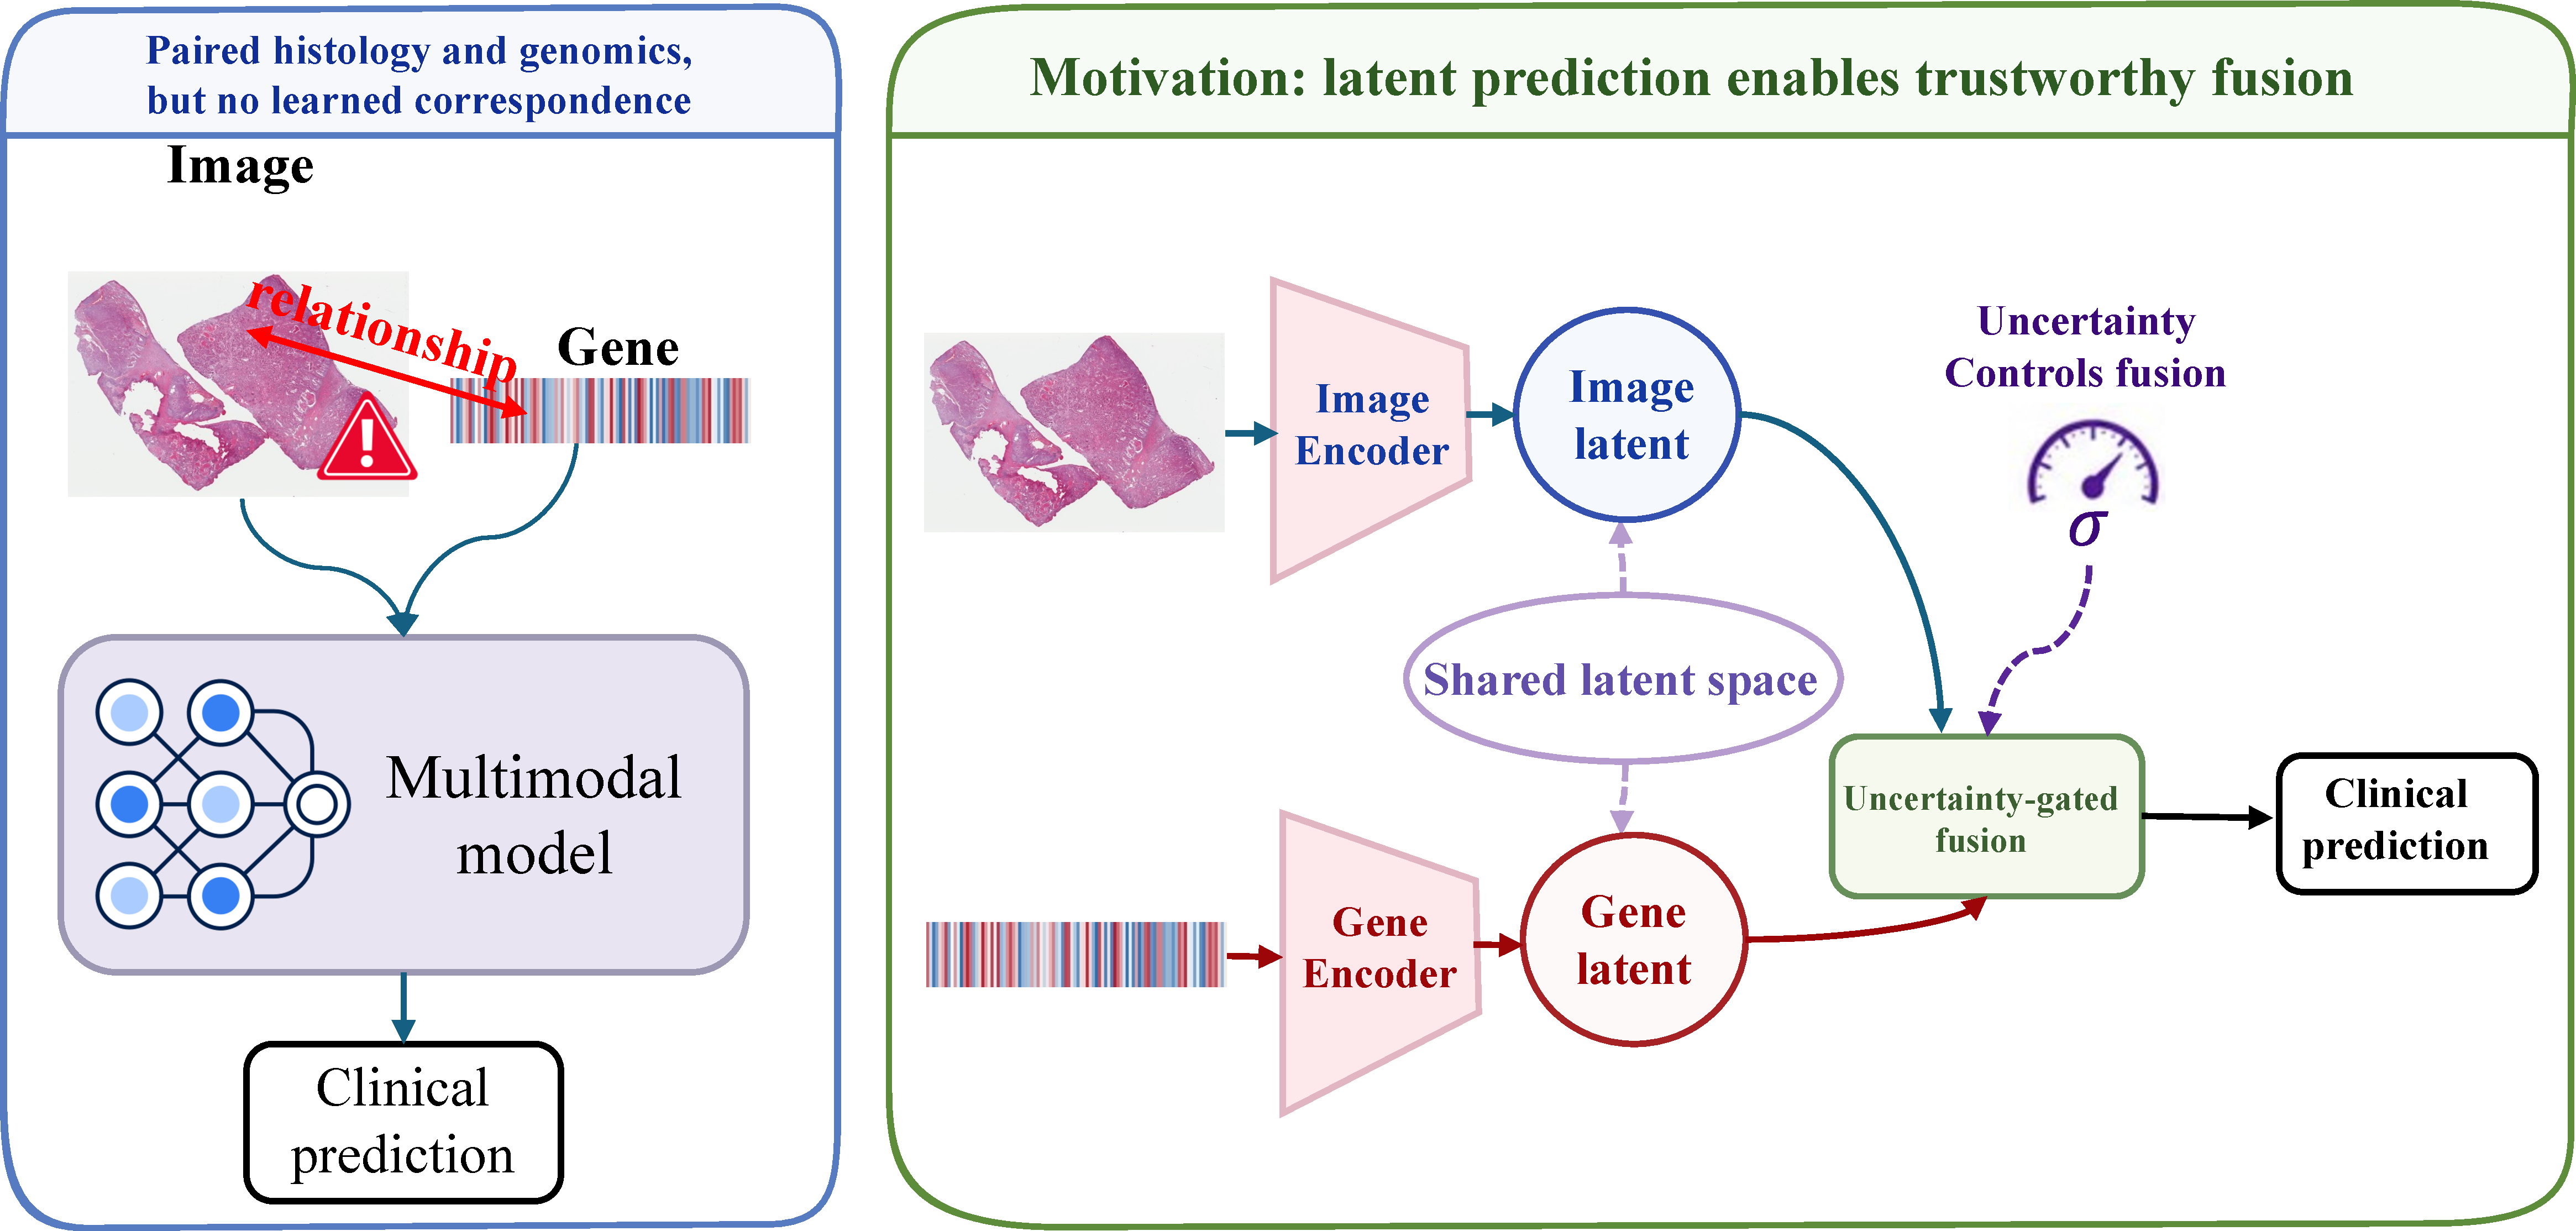
\includegraphics[width=0.8\linewidth]{figures/fig1.pdf}
    \caption{\textbf{Motivation.} JPathGene learns bidirectional latent prediction
and uncertainty-guided fusion.}
    \label{fig:overview}
\end{figure}

